\documentclass{ctexart}
\usepackage{PhysicalChemistryNote}

\begin{document}\pagestyle{plain}
\noindent\tbf{\LARGE 7D 反应机理示例}\vspace{15pt}\\
\indent 在这一节中,我们将综合运用你的数学与化学知识来推导各种反应的速率方程,%
并加深你对\tbf{7C}中学习的理论知识的印象与实用的技巧.
\begin{hint}
    需要说明的是,一般我们给出的复杂反应的反应机理中的各步骤都是基元反应.%
    因此你可以大胆地将基元反应的性质与速率方程应用于它们.
\end{hint}\vspace{8pt}
\Section{7D.1 链反应动力学}
\Part{链反应的基本概念}
\indent 在化学动力学中有一类特殊的反应,只需用热,光或辐射等方法使反应引发,%
体系就能通过活性组分(通常是自由基或原子)相继发生一系列的连续反应,%
像链条一样自动地发展下去.
\begin{definition}[7D.1.1 链反应]
    \tbf{链反应}(又称\tbf{连锁反应}),是指反应的产物或副产物又可作为其他反应的原料,%
    从而使反应反复发生.在化学中,链反应通常在光,热,辐射或引发剂作用下,反应中交替产生活性中间体(如自由原子或自由基),%
    从而使反应一直进行下去.
\end{definition}
按照活性物质数量的变化,链反应主要有三个过程.
\begin{definition}[7D.1.2 链反应的过程]
    在链反应中,产生活性中间体的过程称为\tbf{链引发},%
    活性中间体与反应物分子反复作用生成产物的过程称为\tbf{链增长}或\tbf{链传递},%
    活性中间体最后湮灭的过程称为\tbf{链终止}.
\end{definition}
一般的链增长过程中,一个活性中间体产生一个新的活性中间体.例如\ce{Cl.}与\ce{H2}的反应:
\begin{tightcenter}
    \ce{Cl. + H2 -> HCl + H.}
\end{tightcenter}
不过,在部分链增长过程中,一个活性中间体也可能产生数个活性中间体.例如\ce{H.}与\ce{O2}的反应:
\begin{tightcenter}
    \ce{H. + O2 -> HO. + O.}
\end{tightcenter}
据此,我们可以按照链增长的性质对链反应进行分类.
\begin{definition}[7D.1.3 直链反应与支链反应]
    一个活性中间体只能产生一个新的活性中间体的反应称为\tbf{直链反应},%
    可以产生两个或多个新的活性中间体的反应称为\tbf{支链反应}.
\end{definition}
我们将在接下来对这些链反应的速率方程进行详细地讨论.\vspace{4pt}\\
\Part{简单直链反应——\ce{H2}与卤素单质的自由基反应}
\indent 对中间体与总反应速率的研究表明,\ce{H2}与\ce{X2}(其中$\ce{X}=\ce{Cl},\ce{Br}$)在光照或加热下的化合反应%
的机理是不同的.我们先从最简单的\ce{H2}与\ce{Cl2}的反应开始.\ce{H2}与\ce{Cl2}通过自由基反应生成\ce{HCl}的反应机理如下.
\begin{tightcenter}
    \ce{Cl2 <=>T[$k_1$][$k_{-1}$] 2Cl.}\\
    \ce{Cl. + H2 ->T[$k_2$] HCl + H.}\\
    \ce{H. + Cl2 ->T[$k_3$] HCl + Cl.}
\end{tightcenter}
由于产物\ce{HCl}十分稳定,因此忽略后两个反应的逆反应.现在我们来推导该体系的反应速率方程.
\begin{derivation}\setcounter{equation}{0}
    体系中的不稳定中间体为\ce{H.}与\ce{Cl.},分别对它们稳态近似有
    \begin{equation}
        \dfrac{\di\con{H.}}{\di t}=k_2\con{Cl.}\con{H2}-k_3\con{H.}\con{Cl2}=0
    \end{equation}
    \begin{equation}
        \dfrac{\di\con{Cl.}}{\di t}=2k_1\con{Cl2}-2k_{-1}\con{Cl.}^2-k_2\con{Cl.}\con{H2}+k_3\con{H.}\con{Cl2}=0
    \end{equation}
    将(2)减去(1)可得
    \begin{equation}
        2k_1\con{Cl2}-2k_{-1}\con{Cl.}^2=0
    \end{equation}
    于是
    \begin{equation}
        \con{Cl.}=\sqrt{\dfrac{k_1}{k_{-1}}\con{Cl2}}
    \end{equation}
    由(1)可得
    \begin{equation}
        \dfrac{\di\con{HCl}}{\di t}=k_2\con{Cl.}\con{H2}+k_3\con{H.}\con{Cl2}=2k_2\con{Cl.}\con{H2}
    \end{equation}
    将(4)代入(5)可得
    \begin{equation}
        \dfrac{\di\con{HCl}}{\di t}=2k_2\con{Cl.}\con{H2}=2k_2\sqrt{\dfrac{k_1}{k_{-1}}}\con{H2}\con{Cl2}^{\frac12}
    \end{equation}
    因此反应对\ce{H2}为一级,对\ce{Cl2}为二分之一级.
\end{derivation}
而\ce{H2}与\ce{Br2}的反应就略微复杂一些.两者通过自由基反应生成\ce{HBr}的反应机理如下.
\begin{tightcenter}
    \ce{Br2 <=>T[$k_1$][$k_{-1}$] 2Br.}\\
    \ce{Br. + H2 <=>T[$k_2$][$k_{-2}$] HBr + H.}\\
    \ce{H. + Br2 ->T[$k_3$] HBr + Br.}
\end{tightcenter}
由于\ce{HBr}相对不那么稳定,并且\ce{H.}的能量很高,因此相比\ce{HCl}需要额外考虑%
\ce{HBr}与\ce{H.}的反应.
\begin{derivation}\setcounter{equation}{0}
    体系中的不稳定中间体为\ce{H.}与\ce{Br.},分别对它们稳态近似有
    \begin{equation}
        \dfrac{\di\con{H.}}{\di t}=k_2\con{Br.}\con{H2}-k_{-2}\con{H.}\con{HBr}-k_3\con{H.}\con{Br2}=0
    \end{equation}
    \begin{equation}
        \dfrac{\di\con{Br.}}{\di t}=2k_1\con{Br2}-2k_{-1}\con{Br.}^2-k_2\con{Br.}\con{H2}+k_{-2}\con{H.}\con{HBr}+k_3\con{H.}\con{Br2}=0
    \end{equation}
    将(2)减去(1)可得
    \begin{equation}
        2k_1\con{Br2}-2k_{-1}\con{Br.}^2=0
    \end{equation}
    于是
    \begin{equation}
        \con{Br.}=\sqrt{\dfrac{k_1}{k_{-1}}\con{Br2}}
    \end{equation}
    将(4)代入(1)可得
    \begin{equation}
        \con{H.}=\dfrac{k_2\con{Br.}\con{H2}}{k_{-2}\con{HBr}+k_3\con{Br2}}=\dfrac{k_2\sqrt{\dfrac{k_1}{k_{-1}}}\con{H2}\con{Br2}^{\frac12}}{k_{-2}\con{HBr}+k_3\con{Br2}}
    \end{equation}
    将(4)(5)代入$\dfrac{\di\con{HBr}}{\di t}$可得
    \begin{equation}
        \dfrac{\di\con{HBr}}{\di t}=k_2\con{Br.}\con{H2}+k_3\con{H.}\con{Br2}-k_{-2}\con{HBr}\con{H.}=\dfrac{2k_2k_3\sqrt{\dfrac{k_1}{k_{-1}}}\con{H2}\con{Br2}^{\frac32}}{k_3\con{Br2}+k_{-2}\con{HBr}}
    \end{equation}
    令$k_a=2k_3\sqrt{\dfrac{k_1}{k_{-1}}},k_b=\dfrac{k_{-2}}{k_2}$,就有
    \begin{equation}
        \dfrac{\di\con{HBr}}{\di t}=\dfrac{k_a\con{H2}\con{Br2}^{\frac32}}{\con{Br2}+k_b\con{HBr}}
    \end{equation}
    这就是我们在\tbf{7A.2}中给出的速率方程.
\end{derivation}
而\ce{H2}与\ce{F2}或\ce{I2}的反应则比较复杂,我们在这里就不叙述了.如果你感兴趣,可以自行查阅相关资料.\vspace{4pt}\\
\Part{复杂直链反应——自由基氧化}
\indent 脂类物质的氧化是油脂保存过程中广泛存在的问题.如果反应物记作\ce{RH},那么总反应方程式如下.
\begin{tightcenter}
    \ce{RH + O2 -> ROOH}
\end{tightcenter}
产生的过氧化物\ce{ROOH}可以进一步催化体系中其余\ce{RH}被\ce{O2}氧化.%
反应的机理如下.
\begin{tightcenter}
    \ce{2ROOH ->T[$k_1$] 2R. + \text{副产物}}\\
    \ce{R. + O2 ->T[$k_2$] ROO.}\\
    \ce{ROO. + RH ->T[$k_3$] ROOH + R.}\\
    \ce{2R. ->T[$k_4$] R2}\\
    \ce{R. + ROO. ->T[$k_5$] ROOR}\\
    \ce{2ROO. ->T[$k_6$] ROOR + O2}
\end{tightcenter}
实验表明有近似关系$4k_4k_6=k_5^2$.%
现在我们来考察这一自催化体系的速率方程(以\ce{O2}的消耗速率计).如果同时考虑三种链终止的方式,%
那么这对我们来说有些复杂,因此我们先从简单的情形入手.\\
\indent \tbf{Case I.} \ce{O2}浓度较低.
\begin{derivation}\setcounter{equation}{0}
    这时,体系中主要存在的自由基为\ce{R.},链终止步骤主要为\ce{2R. -> R2}.对体系中的两种自由基\ce{R.}和\ce{ROO.}做稳态近似可得
    \begin{equation}
        \dfrac{\di\con{R.}}{\di t}=2k_1\con{ROOH}^2-k_2\con{R.}\con{O2}+k_3\con{ROO.}\con{RH}-2k_4\con{R.}^2=0
    \end{equation}
    \begin{equation}
        \dfrac{\di\con{ROO.}}{\di t}=k_2\con{R.}\con{O2}-k_3\con{ROO.}\con{RH}=0
    \end{equation}
    $(1)-(2)$可得
    \begin{equation}
        2k_1\con{ROOH}^2-2k_4\con{R.}^2=0
    \end{equation}
    于是
    \begin{equation}
        \con{R.}=\sqrt{\dfrac{k_1}{k_4}}\con{ROOH}
    \end{equation}
    于是
    \begin{equation}
        -\dfrac{\di\con{O2}}{\di t}=k_2\con{R.}\con{O2}=k_2\sqrt{\dfrac{k_1}{k_4}}\con{ROOH}\con{O2}
    \end{equation}
    此时,反应对\ce{ROOH}和\ce{O2}均为一级.可以看到,%
    反应的速率随着产物\ce{ROOH}的增加而增加,因此随着反应进行,速率会逐渐加快.
\end{derivation}
\tbf{Case II.} \ce{O2}浓度较高.
\begin{derivation}\setcounter{equation}{0}
    这时,体系中主要存在的自由基为\ce{ROO.},链终止步骤主要为\ce{2ROO. -> ROOR + O2}.对体系中的两种自由基\ce{R.}和\ce{ROO.}做稳态近似可得
    \begin{equation}
        \dfrac{\di\con{R.}}{\di t}=2k_1\con{ROOH}^2-k_2\con{R.}\con{O2}+k_3\con{ROO.}\con{RH}=0
    \end{equation}
    \begin{equation}
        \dfrac{\di\con{ROO.}}{\di t}=k_2\con{R.}\con{O2}-k_3\con{ROO.}\con{RH}-2k_6\con{ROO.}^2=0
    \end{equation}
    $(1)+(2)$可得
    \begin{equation}
        2k_1\con{ROOH}^2-2k_6\con{ROO.}^2=0
    \end{equation}
    于是
    \begin{equation}
        \con{ROO.}=\sqrt{\dfrac{k_1}{k_6}}\con{ROOH}
    \end{equation}
    由(2)亦可得
    \begin{equation}
        -\dfrac{\di\con{O2}}{\di t}=k_2\con{R.}\con{O2}-k_6\con{ROO.}^2=k_3\con{ROO.}\con{RH}+k_6\con{ROO.}^2
    \end{equation}
    由于自由基\ce{ROO.}的浓度很低,链终止的速率远小于链增长的速率,因此可以近似地忽略后一项.于是有
    \begin{equation}
        -\dfrac{\di\con{O2}}{\di t}=k_3\sqrt{\dfrac{k_1}{k_6}}\con{ROOH}\con{RH}
    \end{equation}
    此时,反应对\ce{ROOH}和\ce{RH}均为一级.可以看到,%
    反应的速率同样随着产物\ce{ROOH}的增加而增加,因此随着反应进行,速率会逐渐加快.
\end{derivation}
在前面两种情况的推导过程中,我们都由稳态近似得出了一个重要的结论.
\begin{theorem}[7D.1.4 直链反应的性质]
    一般而言,如果对反应采取稳态近似处理,那么直链反应中链引发和链终止的速率相等.
\end{theorem}
这是因为我们总是假设体系内所有自由基的浓度随时间变化都不大,因而自由基的总浓度可以近似看作不变.%
对于直链反应而言,链转移不改变自由基数目,只有链引发和链终止可以改变,因而这两个反应的速率近似相同.\\
\indent \tbf{Case III. }一般情形.
\begin{derivation}\setcounter{equation}{0}
    我们仍然对\ce{R.}和\ce{ROO.}稳态近似可得
    \begin{equation}
        \dfrac{\di\con{R.}}{\di t}=2k_1\con{ROOH}^2-k_2\con{R.}\con{O2}+k_3\con{ROO.}\con{RH}-2k_4\con{R.}^2-k_5\con{R.}\con{ROO.}=0
    \end{equation}
    \begin{equation}
        \dfrac{\di\con{ROO.}}{\di t}=k_2\con{R.}\con{O2}-k_3\con{ROO.}\con{RH}-k_5\con{R.}\con{ROO.}-2k_6\con{ROO.}^2=0
    \end{equation}
    $(1)+(2)$可得
    \begin{equation}
        k_1\con{ROOH}^2=k_4\con{R.}^2+k_5\con{R.}\con{ROO.}+k_6\con{ROO.}^2
    \end{equation}
    这也与\tbf{7D.1.4}的结论符合.\\
    体系内的变量仍然太多,因此我们需要进一步做一些合理的近似.%
    考虑到链引发和链终止的速率应当远小于链转移的速率,于是对于(1)或(2)有
    \begin{equation}
        k_2\con{R.}\con{O2}=k_3\con{ROO.}\con{RH}
    \end{equation}
    即
    \begin{equation}
        \con{ROO.}=\dfrac{k_2\con{O2}}{k_3\con{RH}}\con{R.}
    \end{equation}
    将(5)代入(3)可得
    \begin{equation}
        k_1\con{ROOH}^2=\left(k_4+\dfrac{k_2\con{O2}}{k_3\con{RH}}k_5+\left(\dfrac{k_2\con{O2}}{k_3\con{RH}}\right)^2k_6\right)\con{R.}^2
    \end{equation}
    我们迫切地希望大括号内也是完全平方式,这样就可以将两边开方以极大地化简.考虑该式的形式,将$k_5=2\sqrt{k_4k_6}$代入(6)可得
    \begin{equation}
        k_1\con{ROOH}^2=\left(k_4+\dfrac{k_2\con{O2}}{k_3\con{RH}}2\sqrt{k_4k_6}+\left(\dfrac{k_2\con{O2}}{k_3\con{RH}}\right)^2k_6\right)\con{R.}^2
    \end{equation}
    这恰好可以改写为完全平方式,即
    \begin{equation}
        k_1\con{ROOH}^2=\left(\sqrt{k_4}+\dfrac{k_2\con{O2}}{k_3\con{RH}}\sqrt{k_6}\right)^2\con{R.}^2
    \end{equation}
    开方后整理可得
    \begin{equation}
        \con{R.}=\dfrac{\sqrt{k_1}\con{ROOH}}{\sqrt{k_4}+\dfrac{k_2\con{O2}}{k_3\con{RH}}\sqrt{k_6}}
    \end{equation}
    于是消耗\ce{O2}的速率
    \begin{equation}
        -\dfrac{\di\con{O2}}{\di t}=k_2\con{R.}\con{O2}=\dfrac{\sqrt{k_1}k_2\con{ROOH}\con{RH}\con{O2}}{\sqrt{k_4}+\dfrac{k_2\con{O2}}{k_3\con{RH}}\sqrt{k_6}}
    \end{equation}
    令$k=k_3\sqrt{\dfrac{k_1}{k_6}},\lambda=\dfrac{k_2}{k_3}\sqrt{\dfrac{k_4}{k_6}}$,就有
    \begin{equation}
        -\dfrac{\di\con{O2}}{\di t}=k\con{ROOH}\dfrac{\con{O2}\con{RH}}{\con{O2}+\lambda\con{RH}}
    \end{equation}
    这也与实验测得的速率方程相符合.
\end{derivation}
\Part{支链反应——\ce{H2}与\ce{O2}的自由基反应}
\indent 我们知道,一定浓度的\ce{H2}与\ce{O2}混合后点燃,有时可以稳定地燃烧,%
有时则会发生剧烈的爆炸.两者的反应通过支链反应进行,其机理可以表述如下.
\begin{tightcenter}
    \ce{H2 ->T[$k_1$] 2H.}\\
    \ce{H. + O2 ->T[$k_2$] HO. + O.}\\
    \ce{O. + H2 ->T[$k_3$] HO. + H.}\\
    \ce{HO. + H2 ->T[$k_4$] H2O + H.}\\
    \ce{H. + M ->T[$k_5$] \text{销毁}}\\
    \ce{H. + O2 + M ->T[$k_6$] \text{销毁}}
\end{tightcenter}
销毁主要是自由基与撞击器壁\ce{M}所致.反应中,\ce{O.}和\ce{HO.}可以作为不稳定中间体,%
而\ce{H.}的浓度则随着反应条件不同而有着不同的变化趋势.%
据此,我们来推导不同条件时反应的速率方程.
\begin{derivation}\setcounter{equation}{0}
    对\ce{O.}和\ce{HO.}稳态近似可得
    \begin{equation}
        \dfrac{\di\con{O.}}{\di t}=k_2\con{H.}\con{O2}-k_3\con{O.}\con{H2}=0
    \end{equation}
    \begin{equation}
        \dfrac{\di\con{HO.}}{\di t}=k_2\con{H.}\con{O2}+k_3\con{O.}\con{H2}-k_4\con{HO.}\con{H2}=0
    \end{equation}
    于是分别可得
    \begin{equation}
        \con{O.}=\dfrac{k_2\con{H.}\con{O2}}{k_3\con{H2}}
    \end{equation}
    \begin{equation}
        \con{HO.}
        =\dfrac{k_2\con{H.}\con{O2}+k_3\con{O.}\con{H2}}{k_4\con{H2}}
        =\dfrac{2k_2\con{H.}\con{O2}}{k_4\con{H2}}
    \end{equation}
    于是可以写出\ce{H.}的生成速率,即
    \begin{equation}
        \begin{aligned}
            \dfrac{\di\con{H.}}{\di t}
            &= 2k_1\con{H2}-k_2\con{H.}\con{O2}+k_3\con{O.}\con{H2}+k_4\con{HO.}\con{H2}-k_5\con{H.}-k_6\con{H.}\con{O2} \\
            &= 2k_1\con{H2}+2k_2\con{H.}\con{O2}-k_5\con{H.}-k_6\con{H.}\con{O2} \\
            &= 2k_1\con{H2}+\left(2k_2\con{O2}-k_5-k_6\con{O2}\right)\con{H.}
        \end{aligned}
    \end{equation}
    可以看到,$\con{H.}$前的项各有正负.不难理解,正项代表\ce{H.}增多的支链增长反应,负项代表\ce{H.}减少的链终止反应.\\
    令$v_i=2k_1\con{H2}$为链引发速率,$k_b=2k_2\con{O2}$为支链化速率常数,$k_t=k_5+k_6\con{O2}$为链终止速率常数,则有
    \begin{equation}
        \dfrac{\di\con{H.}}{\di t}=v_i+\left(k_b-k_t\right)\con{H.}
    \end{equation}
    在反应的初始阶段,\ce{H2}与\ce{O2}的浓度变化都不大,可以将$v_0,k_b$和$k_t$都视作常数.对(6)移项积分可得
    \begin{equation}
        \con{H.}=\dfrac{v_i}{k_b-k_t}\left(\e^{\left(k_b-k_t\right)t}-1\right)
    \end{equation}
    这就是反应初期$\con{H.}$与时间$t$的关系.
\end{derivation}
显然,上面的(7)式会由于$k_b-k_t$的大小显现出不同的关系.我们将图像绘制如下.
\begin{figure}[H]
    \centering\documentclass{standalone}
\usepackage{PhysicalChemistryNote}
\begin{document}
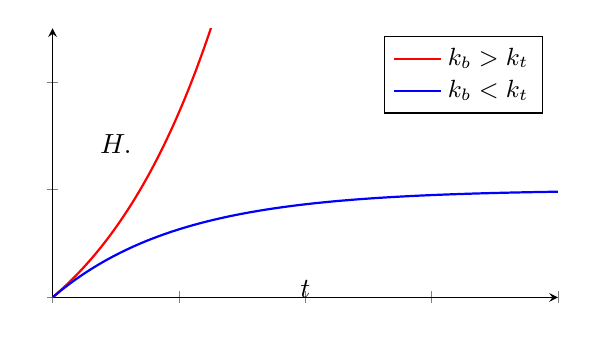
\begin{tikzpicture}
    \begin{axis}[
        width = 8cm,
        height = 5cm,
        legend pos = north east,
        x label style={at={(axis description cs:0.5,0.1)},anchor=north},
        y label style={at={(axis description cs:0.125,0.5)},rotate=270,anchor=south},
        xlabel = {$t$},
        ylabel = {$\con{H.}$},
        axis lines = left,
        ymax = 5,
        domain = 0:8,
        samples = 400,
        xticklabels={},
        yticklabels={}
    ]
    \addplot [thick, red] {2*(e^(0.5*x)-1)};
    \addlegendentry{\small{$k_b>k_t$}}
    \addplot [thick, blue] {-2*(e^(-0.5*x)-1)};
    \addlegendentry{\small{$k_b<k_t$}}
    \end{axis}
\end{tikzpicture}
\end{document}
\end{figure}
可以看到,当$k_b>k_t$时,\ce{H.}的浓度随时间指数增长,反应将在很短的时间发生,最终表现为爆炸.%
当$k_b<k_t$时,\ce{H.}的浓度随着时间增长趋于平稳,反应的速率为一常数,最终表现为稳定燃烧.\vspace{12pt}\\
\Section{7D.2 聚合反应动力学}
\indent 聚合反应是把低分子量的单体转化成高分子量的聚合物的过程,%
聚合物具有低分子量单体所不具备的可塑性等重要性能,可广泛地用作塑料,纤维,橡胶,涂料,黏合剂等用途.%
聚合物是由一种以上的结构单元(单体)构成的,由单体经重复反应合成的高分子化合物.\\
\indent 聚合反应最特殊的一点在于,我们一般不以产物浓度衡量反应进行的状况,转而用聚合度这一概念.
\begin{definition}[7D.2.1 聚合度]
    \tbf{聚合度}即每个聚合物分子中留存的单体的平均数目,记作$DP$.
\end{definition}
根据机理的不同,我们可以将聚合反应分为如下两类.
\begin{definition}[7D.2.2 逐步聚合与链聚合]
    \tbf{逐步聚合}是指带有两个或多个官能团的单体相互反应,逐步生成二聚体,三聚体,寡聚物以最终形成高分子聚合物的聚合反应.%
    缩聚反应一般通过逐步聚合进行.\\
    \tbf{链聚合}是指中间体与单体反应,每次增长一个长度的聚合反应.%
    加聚反应一般通过链聚合进行,这其中最典型的是自由基链聚合.
\end{definition}
我们先来考虑逐步聚合的速率方程.为了简便考虑,假定只有一种单体参与逐步聚合.%
不妨假定是羟基羧酸\ce{HO-R-COOH}发生缩聚反应.我们现在来推导这一聚合反应的速率方程.
\begin{derivation}
    直接考虑聚合过程显然有些麻烦,因为任意长度的两条链都有可能发生反应形成一条新的链.%
    但有一点是可以确定的,即每一次反应都会使得\ce{-OH}和\ce{COOH}减少一个.因此,%
    我们可以考虑用\ce{-COOH}官能团(记作\ce{A})的浓度衡量反应的进度.\\
    一般的酯化反应对于醇和羧酸均为一级,即
    \[v=k\con{R_1OH}\con{R_2COOH}\]
    对于\ce{HO-R-COOH}而言,每个分子(以及聚合形成的链)都有一个\ce{-COOH}和\ce{-OH},因此有
    \[v=-\dfrac{\di\con{A}}{\di t}=k\con{A}^2\]
    这是一个典型的二级反应,由\tbf{7B.1.5}可知它的积分速率方程
    \[\con{A}=\dfrac{\con{A}_0}{1+k\con{A}_0t}\]
    由于每个聚合物分子都仅在端基含有一个\ce{-COOH},因此聚合物的平均链长与\ce{-COOH}的数目的乘积应当是定值.%
    反应开始时体系中均为单体,聚合度为$1$.于是就有
    \[DP\cdot\con{A}=\con{A}_0\]
    于是
    \[DP=\dfrac{\con{A}_0}{\con{A}}=1+k\con{A}_0t\]
    可见聚合度随着时间线性增长.\\
    我们也可以使用尚未参与反应的\ce{A}的比例$p$衡量聚合反应进行的程度.这样就有
    \[p=\dfrac{\con{A}_0-\con{A}}{\con{A}_0}=\dfrac{k\con{A}_0t}{1+k\con{A}_0t}\]
    以及
    \[DP=\dfrac{1}{1-p}\]

\end{derivation}
这样,我们就知道在这样的简单逐步聚合中,聚合度随时间线性增长这一事实.%
如果你对更加复杂的体系(例如有多种反应物)感兴趣,也可以用相似的步骤推导它们的速率方程.\\
\indent 我们在前面还给出了聚合度$DP$与反应程度$p$的关系,即$D=\dfrac{1}{1-p}$.%
Carothers于1935年提出了在各种体系中$DP$与$p$的关系.
\begin{theorem}[7D.2.3 Carothers方程]
    逐步聚合中,两种等物质的量的单体形成完全线性的聚合物(或者一种单体自身聚合)时,%
    聚合度$DP$与反应程度$p$满足
    \[DP=\dfrac{1}{1-p}\]
    如果一种单体相对过量,则有
    \[DP=\dfrac{1+r}{1+r-2rp}\]
    其中$r$是较少量单体和较多单体的基团比或物质的量之比.
\end{theorem}
你可以自行推导上述结论.\\
\indent 现在,我们来考虑另一种聚合机理——链聚合.它的过程与我们在\tbf{7D.1}中提到的直链反应十分相似,%
我们假定引发剂为\ce{In},聚合单体为\ce{M},则反应机理可以表述如下.
\begin{tightcenter}
    \ce{In ->T[$k_i$] 2R.}\\
    \ce{M + R. ->T[fast] M_1.}\\
    \ce{M_{$n$}. + M ->T[$k_p$] M_{$n+1$}.}\\
    \ce{M_{$n$}. + M_{$m$}. ->T[$k_t$] M_{$n+m$}}
\end{tightcenter}
引发剂形成的自由基\ce{R.}由于其高活泼性,容易在与\ce{M}反应之前就发生分解.%
因此,我们设参与第二个反应的\ce{R.}的比例为$f$.同时,为了简化体系,我们在链终止中只考虑偶联终止.现在我们来推导体系的速率方程.
\begin{derivation}
    我们记\ce{M.}为体系中任意长度的聚合物中间体(这是推导过程中最重要的一步,由于不同长度的中间体在动力学上并无显著不同,因此我们可以将它们视同一种物质).\\
    引发过程的决速步为引发剂\ce{In}的裂解;链增长步骤不改变\ce{M.}的总浓度.因此,对\ce{M.}稳态近似可得
    \[\dfrac{\di\con{M.}}{\di t}=2fk_i\con{In}-2k_t\con{M.}^2\]
    从而
    \[\con{M.}=\sqrt{\dfrac{fk_i\con{In}}{k_t}}\]
    \ce{M}主要在链增长过程中被消耗,于是其消耗速率
    \[-\dfrac{\di\con{M}}{\di t}=k_p\con{M.}\con{M}=k_p\sqrt{\dfrac{fk_i}{k_t}}\con{M}\con{In}^{\frac12}\]
    现在考虑聚合物的链长.我们先不考虑终止方式,仅考虑引发与增长过程.%
    显然,在链增长时被消耗的\ce{M}的数目与用于引发的\ce{R.}的数目之比就是每个链在终止之前的平均长度.我们把它记为动力学链长$\lambda$,即有
    \[\lambda
    =\dfrac{n\left(\text{消耗的\ce{M}}\right)}{n\left(\text{用于引发的\ce{R.}}\right)}
    =\dfrac{v\left(\text{链增长}\right)}{v\left(\text{链引发}\right)}
    =\dfrac{v\left(\text{链增长}\right)}{v\left(\text{链终止}\right)}
    =\dfrac{k_p\con{M.}\con{M}}{2k_t\con{M.}^2}
    =\dfrac{k_p\con{M}}{2k_t\con{M.}}\]
    代入$\con{M.}$的表达式即有
    \[\lambda=\dfrac{k_p}{2\sqrt{fk_ik_t}}\con{M}\con{In}^{-\frac12}\]
    由于这里的终止方式是偶联终止,因此产物事实上由两条链构成.于是聚合度
    \[DP=2\lambda=\dfrac{k_p}{\sqrt{fk_ik_t}}\con{M}\con{In}^{-\frac12}\]
    这就是链聚合的聚合度的表达式.对于不同的引发剂和终止方式,上式略有不同,%
    但整体上的推导方式是相似的.\\
    从上式也可以看出,单体\ce{M}的浓度越高,引发剂\ce{In}的浓度越低,聚合度越大.
\end{derivation}\vspace{8pt}
\Section{7D.3 酶促反应动力学}
\indent 迄今为止,我们还没有系统地讨论有催化剂参与时反应的动力学特征.%
尽管在前面,我们已经讨论了一类自催化反应,但大多数时候催化剂都是额外加入的,在总反应中不会被消耗的物质.\\
\indent 我们在本节要讨论的催化剂,\tbf{酶},就是一种高效专一的生物均相催化剂.关于酶的基本概念与特性,你可以查阅生物化学书.%
我们在这里主要关注酶催化的反应,即\tbf{酶促反应}的动力学特性.\vspace{4pt}\\
\Part{简单酶促反应与米氏方程}
\indent 最简单的酶催化反应的机理可由以下基元反应描述.
\begin{tightcenter}
    \ce{E + S <=>T[$k_1$][$k_{-1}$] ES ->T[$k_2$] E + P}
\end{tightcenter}
其中\ce{E}即参与催化的酶,\ce{S}为底物(即反应物),\ce{ES}为酶-底物复合中间体,\ce{P}为产物.%
我们现在来推导该反应的速率方程.
\begin{derivation}
    对中间体\ce{ES}做稳态近似可得
    \[\dfrac{\di\con{ES}}{\di t}=k_1\con{E}\con{S}-k_{-1}\con{ES}-k_2\con{ES}=0\]
    于是有
    \[\con{ES}=\dfrac{k_1\con{E}\con{S}}{k_{-1}+k_2}\]
    根据催化剂的物料守恒可得
    \[\con{E}+\con{ES}=\con{E}_0\]
    于是
    \[\con{E}=\dfrac{\con{E}_0}{1+\dfrac{k_1\con{S}}{k_{-1}+k_2}}\ \ \ \ \ 
    \con{ES}=\dfrac{k_1\con{E}_0\con{S}}{k_{-1}+k_2+k_1\con{S}}\]
    于是反应的速率即为
    \[\dfrac{\di\con{P}}{\di t}=k_2\con{ES}=\dfrac{k_1k_2\con{E}_0\con{S}}{k_{-1}+k_2+k_1\con{S}}\]
    为了简化上式,我们不妨定义$K_M=\dfrac{k_{-1}+k_2}{k_1}$,这样就有
    \[\con{ES}=\dfrac{\con{E}\con{S}}{K_M}\]
    同理,最后可以得出
    \[\dfrac{\di\con{P}}{\di t}=\dfrac{k_2\con{E}_0}{1+\dfrac{K_M}{\con{S}}}\]
    如果底物\ce{S}大大过量,那么就有$\dfrac{K_M}{\con{S}}\sim0$,于是
    \[\dfrac{\di\con{P}}{\di t}=\dfrac{k_2\con{E}_0}{1+\dfrac{K_M}{\con{S}}}\approx k_2\con{E}_0\]
    这就是酶的总浓度一定时反应的最大速率,记作$v_{\max}$.如此,速率方程亦可以写作
    \[v=\dfrac{v_{\max}}{1+\dfrac{K_M}{\con{S}}}\]
    
\end{derivation}
这就是Leonor Michaelis和Maud Menten提出的\tbf{米氏方程}.
\begin{theorem}[7D.3.1 米氏方程]
    对于符合
    \begin{tightcenter}
        \ce{E + S <=>T[$k_1$][$k_{-1}$] ES ->T[$k_2$] E + P}
    \end{tightcenter}
    机理的酶促反应,其速率方程为
    \[v=\dfrac{v_{\max}}{1+\dfrac{K_M}{\con{S}}}\]
    其中\tbf{米氏常数}$K_M=\dfrac{k_{-1}+k_2}{k_1}$.$v_{\max}=k_2\con{E}_0$,是该反应在酶的总浓度$\con{E}_0$一定时能达到的最大速率.
\end{theorem}
以下是$v$对$\con{S}$作图的结果.可以看出,当$\con{S}\ll K_M$时近似地有$v=\dfrac{v_{\max}}{K_M}\con{S}$,反应对\ce{S}为准一级.%
当$\con{S}\gg K_M$时,反应速率趋近于$v_{\max}$,反应对$\con{S}$为准零级.
\begin{tightcenter}
    \documentclass{standalone}
\usepackage{PhysicalChemistryNote}
\begin{document}
\begin{tikzpicture}
    \draw[->] (0,0)--(6,0) node[right]{$\con{S}$};
    \draw[->] (0,0)--(0,4.5) node[above]{$v$};
    \draw[domain=0.0001:6] plot[smooth](\x,{4/(1+0.5/\x)});
    \draw[dashed] (0,4)--(6,4);
    \fill (0,4) circle (1.5pt) node[left]{$v_{\max}$};
\end{tikzpicture}
\end{document}
\end{tightcenter}
\indent 反应速率常数$k_1,k_{-1},k_2$是较难直接获取的,但米氏方程为我们提供了线性回归测定它们的方式.%
将米氏方程变形可得
\[\dfrac{1}{v}=\dfrac{1}{v_{\max}}+\left(\dfrac{K_M}{v_{\max}}\right)\dfrac{1}{\con{S}}\]
可以看到,$\dfrac{1}{v}$与$\dfrac{1}{\con{S}}$成一次函数关系.测定\ce{S}在不同起始浓度$\con{S}_0$及其对应的速率$v_0$,%
就可以通过线性回归的方式求出斜率$\dfrac{K_M}{v_{\max}}$和截距\footnote{如无特别说明,截距一般指$y$轴截距.}$\dfrac{1}{v_{\max}}$.%
这种方式就是\tbf{Lineweaver-Burk作图法}\footnotemark\footnotetext{分别译作“莱恩威弗-伯克作图法”,“哈尼斯-伍尔夫作图法”和“伊迪-霍夫斯蒂作图法”.}.
\begin{theorem}[7D.3.2 Lineweaver-Burk作图法]
    在符合米氏方程的酶促反应中,反应速率的倒数$\dfrac1v$和底物浓度$\dfrac{1}{\con{S}}$成一次函数关系,根据实验数据作图就可以求得米氏常数$K_M$.%
    因此,这一方法也被称作\tbf{双倒数法}.
\end{theorem}
下面是由Lineweaver-Burk作图法给出\tbf{7D.3.1}的图像.
\begin{tightcenter}
    \documentclass{standalone}
\usepackage{PhysicalChemistryNote}
\begin{document}
\begin{tikzpicture}
    \draw[->] (-2.5,0)--(4,0) node[right]{$\dfrac{1}{\con{S}}$};
    \draw[->] (0,0)--(0,3.5) node[left]{$\dfrac{1}{v}$};
    \draw[dashed] (-2,0)--(1,1.5);
    \draw[-] (1,1.5)--(4,3);
    \fill (0,1) circle (1.5pt) node[above left]{\small{$\dfrac{1}{v_{\max}}$}};
    \fill (-2,0) circle (1.5pt) node[below]{\small{$-\dfrac{1}{K_M}$}};
    \node at (2,0.5) {\small{$\dfrac{1}{v}=\dfrac{1}{v_{\max}}+\left(\dfrac{K_M}{v_{\max}}\right)\dfrac{1}{\con{S}}$}};
\end{tikzpicture}
\end{document}
\end{tightcenter}
通过$x$轴截距和$y$轴截距就能计算出$v_{\max}$和$K_{M}$.%
不过,这一方法仍不能给出$k_1$和$k_{-1}$的具体值.%
我们需要更复杂的手段进行测量,这里就不再赘述.\\
\indent Lineweaver-Burk作图法仍然存在一些缺陷.只有当$\con{S}$相当小时,我们才能获取远离$y$轴的数据点.%
对于一般浓度的\ce{S},对应的数据大多靠近$y$轴,较为密集,在线性回归时容易引起误差.因此,可以对作图的直线表达式两端同乘$\con{S}$,即有
\[\dfrac{\con{S}}{v}=\dfrac{\con{S}}{v_{\max}}+\dfrac{K_{M}}{v_{\max}}\]
通过$\dfrac{\con{S}}{v}$对$\con{S}$作图,得到斜率为$\dfrac{1}{v_{\max}}$,截距为$\dfrac{K_M}{v_{\max}}$的直线.这就是\tbf{Hanes-Woolf作图法}\footnotemark[\arabic{footnote}].\\
\indent 当然,你还可以对\tbf{7D.3.1}变形得到
\[\dfrac{v}{\con{S}}=\dfrac{v_{\max}}{K_M}-\dfrac{v}{K_M}\]
通过$\dfrac{v}{\con{S}}$对$v$作图,得到斜率为$-\dfrac{1}{K_M}$,截距为$\dfrac{v_{\max}}{K_M}$的直线.这就是\tbf{Eadie-Hofstee作图法}\footnotemark[\arabic{footnote}].\vspace{4pt}\\
\Part{竞争性抑制剂和非竞争性抑制剂}
\indent 酶对反应体系是敏感的.一些物质可以与酶发生反应,进而降低其活性或使其完全失效.这就是\tbf{抑制剂}.
\begin{definition}[7D.3.3 抑制剂]
    \tbf{酶抑制剂}是一类特异性作用于或影响酶的活性中心或必需基团,导致酶活性下降或丧失,进而降低酶促反应速率的物质.
\end{definition}
按照抑制剂作用的机理不同,酶抑制剂可以简单地被分为如下两类.
\begin{definition}[7D.3.4 抑制剂的分类]
    \tbf{竞争性抑制剂}在结构上通常与底物相似.它和底物不能同时与酶结合,通常是由于它和底物对酶的同一活性位点都具有亲和力,故底物和抑制剂竞争结合该位点,从而使得反应减缓.\\
    \tbf{非竞争性抑制剂}通常与酶的非活性部位结合,改变酶的结构,从而降低酶的活性,但不影响酶与底物结合.\\
    \tbf{反竞争性抑制剂}仅与酶-底物复合物结合,导致其不能正常发生分解而生成产物.\\
    \tbf{复合抑制剂}可以与酶或酶-底物复合物结合,使得反应的速率减缓.\\
    以上四种抑制剂的结合都是可逆的.\tbf{不可逆抑制剂}通过与酶形成共价键,彻底改变其性质,从而使得反应减缓,并且这一作用是不可逆的.
\end{definition}
我们现在来推导竞争性抑制剂存在下反应的速率方程.这一反应的机理可以表述如下.
\begin{tightcenter}
    \ce{E + S <=>T[$k_1$][$k_{-1}$] ES ->T[$k_2$] E + P}\\
    \ce{E + I <=>T[$k_3$][$k_{-3}$] EI}
\end{tightcenter}
\begin{derivation}
    对\ce{ES}稳态近似,可知仍然满足米氏方程给出的关系
    \[\con{ES}=\dfrac{\con{E}\con{S}}{K_{M}}\]
    另一方面,对\ce{EI}稳态近似可得
    \[\dfrac{\di\con{EI}}{\di t}=k_3\con{E}\con{I}-k_{-3}\con{EI}=0\]
    令$K_{\ce{I}}=\dfrac{k_{-3}}{k_{3}}$为抑制反应的平衡常数的倒数,则有
    \[\con{EI}=\dfrac{\con{E}\con{I}}{K_{\ce{I}}}\]
    由\ce{E}的物料守恒有
    \[\left(1+\dfrac{\con{S}}{K_{M}}+\dfrac{\con{I}}{K_{\ce{I}}}\right)\con{E}=\con{E}_0\]
    于是反应的速率即为
    \[v
    = \dfrac{\di\con{P}}{\di t}=k_2\con{ES}=\dfrac{k_2\con{E}\con{S}}{K_{M}}
    = \dfrac{k_2\con{S}}{K_{M}}\cdot\dfrac{\con{E}_0}{1+\dfrac{\con{S}}{K_{M}}+\dfrac{\con{I}}{K_{\ce{I}}}}
    = \dfrac{k_2\con{E}_0\con{S}}{\con{S}+\left(1+\dfrac{\con{I}}{K_{\ce{I}}}\right)K_{M}}\]
    我们按照Lineweaver-Burk作图法的形式对上式整理可得
    \[\dfrac{1}{v}=\dfrac{1}{v_{\max}}+\dfrac{K_{M}}{v_{\max}}\left(1+\dfrac{\con{I}}{K_{\ce{I}}}\right)\dfrac{1}{\con{S}}\]
    令$\alpha=1+\dfrac{\con{I}}{K_{\ce{I}}}$,则上式可以写作
    \[\dfrac{1}{v}=\dfrac{1}{v_{\max}}+\dfrac{\alpha K_{M}}{v_{\max}}\dfrac{1}{\con{S}}\]
    可见竞争性抑制剂不改变直线的截距,只改变直线的斜率.%
    如果令$\alpha K_M=K_{M,\text{obs}}$为表观米氏常数,就可以知道竞争性抑制剂只改变$K_{M,\text{obs}}$,不改变$v_{\max}$.
\end{derivation}

\indent 反竞争性抑制剂的机理与竞争性抑制剂有些相似,可以表述如下.
\begin{tightcenter}
    \ce{E + S <=>T[$k_1$][$k_{-1}$] ES ->T[$k_2$] E + P}\\
    \ce{ES + I <=>T[$k_3$][$k_{-3}$] ESI}
\end{tightcenter}
我们现在来推导该反应的速率方程.
\begin{derivation}
    综合前面的推导,我们可以容易地得出
    \[\con{E}=\dfrac{K_M}{\con{S}}\con{ES}\ \ \ \ \ \con{ESI}=\dfrac{\con{I}}{K_{\ce{I}}}\con{ES}\]
    其中同样地有$K_{\ce{I}}=\dfrac{k_{-3}}{k_3}$.于是反应的速率为
    \[v=\dfrac{k_2\con{E}_0}{1+\dfrac{\con{I}}{K_{\ce{I}}}+\dfrac{K_M}{\con{S}}}\]
    令$\alpha=1+\dfrac{\con{I}}{K_{\ce{I}}}$.我们按照Lineweaver-Burk作图法的形式对上式整理可得
    \[\dfrac{1}{v}=\dfrac{\alpha}{v_{\max}}+\dfrac{K_M}{v_{\max}}\dfrac{1}{\con{S}}\]
    可见反竞争性抑制剂只改变直线的截距,不改变直线的斜率.它同步地影响$K_{M,\text{obs}}$与$v_{\max}$.
\end{derivation}
非竞争性抑制剂的作用原理则稍复杂一些,它的机理可以表述如下.
\begin{tightcenter}
    \ce{E + S <=>T[$k_1$][$k_{-1}$] ES ->T[$k_2$] E + P}\\
    \ce{E + I <=>T[$k_{3}$][$k_{-3}$] EI}\ \ \ \ \ \ce{ES + I <=>T[$k_4$][$k_{-4}$] ESI}\\
    \ce{EI + S <=>T[$K$] ESI}
\end{tightcenter}
由于体系中的\ce{E},\ce{ES},\ce{EI}和\ce{ESI}处于快速平衡中,因此最后一个反应的平衡常数$K$可以由前面的速率常数求出,%
不是一个独立的量.我们现在来推导该反应的速率方程.
\begin{derivation}
    仍然有
    \[\con{ES}=\dfrac{\con{E}\con{S}}{K_{M}}\]
    同样地,令$K_1=\dfrac{k_{-3}}{k_3},K_2=\dfrac{k_{-4}}{k_4}$分别为两个抑制反应的平衡常数的倒数,根据平衡态假设有
    \[\con{EI}=\dfrac{\con{E}\con{I}}{K_1}\ \ \ \ \ \con{ESI}=\dfrac{\con{ES}\con{I}}{K_2}\]
    根据催化剂的物料守恒可得
    \[\left[\left(1+\dfrac{\con{I}}{K_1}\right)\dfrac{K_M}{\con{S}}+1+\dfrac{\con{I}}{K_2}\right]\con{ES}=\con{E}_0\]
    于是反应的速率为
    \[v=\dfrac{\di\con{P}}{\di t}=k_2\con{ES}=\dfrac{k_2\con{E}_0}{1+\dfrac{\con{I}}{K_2}+\left(1+\dfrac{\con{I}}{K_1}\right)\dfrac{K_M}{\con{S}}}\]
    一般情况下,抑制剂\ce{I}由于结合的位点与活性位点无关,因此\ce{I}与\ce{E}和\ce{ES}的结合能力应当相同,即$K_1=K_2$.令$K_{\ce{I}}=K_1=K_2$,再令$\alpha=1+\dfrac{\con{I}}{K_{\ce{I}}}$,就有
    \[v=\dfrac{k_2\con{E}_0}{\alpha\left(1+\dfrac{K_M}{\con{S}}\right)}\]
    我们按照Lineweaver-Burk作图法的形式对上式整理可得
    \[\dfrac{1}{v}=\dfrac{\alpha}{v_{\max}}+\dfrac{\alpha K_M}{v_{\max}}\dfrac{1}{\con{S}}\]
    如果令$v_{\max}'=\dfrac{v_{\max}}{\alpha}$,就有
    \[\dfrac{1}{v}=\dfrac{1}{v_{\max}'}+\dfrac{K_M}{v_{\max}'}\dfrac{1}{\con{S}}\]
    可见非竞争性抑制剂不改变直线的$x$轴截距,即不改变$K_M$,而只改变$v_{\max}$.
\end{derivation}
我们将这些抑制剂的作用总结如下.
\begin{theorem}[7D.3.5 抑制剂的作用]
    竞争性抑制剂使得$K_{M,\text{obs}}$减小,但不改变$v_{\max}$.\\
    反竞争性抑制剂使得$K_{M,\text{obs}}$和$v_{\max}$都减小,但不改变$\dfrac{K_{M,\text{obs}}}{v_{\max}}$.\\
    非竞争性抑制剂使得$v_{\max}$减小,但不改变$K_{M,\text{obs}}$.
\end{theorem}
我们在下面给出加入这几种抑制剂后的图像和对应的Lineweaver-Burk图以供你参考.
\begin{figure}[H]
    \centering\documentclass{standalone}
\usepackage{PhysicalChemistryNote}
\begin{document}
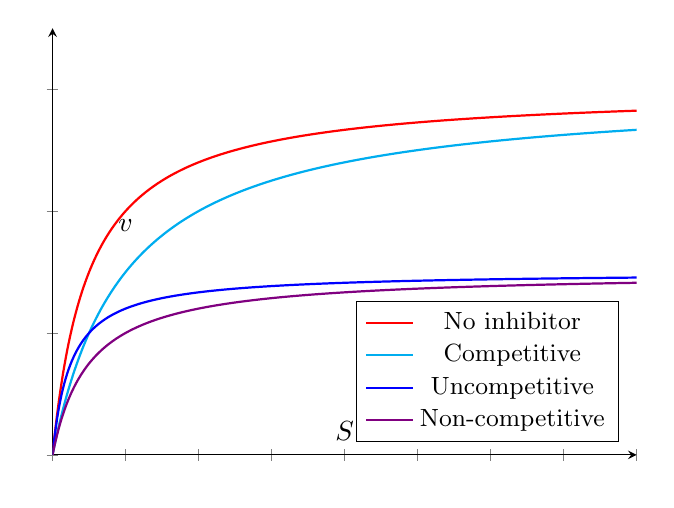
\begin{tikzpicture}
    \begin{axis}[
        width = 9cm,
        height = 7cm,
        legend pos = south east,
        x label style={at={(axis description cs:0.5,0.1)},anchor=north},
        y label style={at={(axis description cs:0.125,0.5)},rotate=270,anchor=south},
        xlabel = {$\con{S}$},
        ylabel = {$v$},
        axis lines = left,
        ymax = 3.5,
        domain = 0:8,
        samples = 400,
        xticklabels={},
        yticklabels={}
    ]
    \addplot [thick, red] {3/(1+0.5/x)};
    \addlegendentry{\small{No inhibitor}}
    \addplot [thick, cyan] {3/(1+1/x)};
    \addlegendentry{\small{Competitive}}
    \addplot [thick, blue] {3/(2+0.5/x)};
    \addlegendentry{\small{Uncompetitive}}
    \addplot [thick, violet] {3/(2+1/x)};
    \addlegendentry{\small{Non-competitive}}
    \end{axis}
\end{tikzpicture}
\end{document}
\end{figure}
\begin{figure}[H]
    \centering\documentclass{standalone}
\usepackage{PhysicalChemistryNote}
\begin{document}
\begin{tikzpicture}
    \begin{axis}[
        width = 9cm,
        height = 6cm,
        legend pos = north east,
        xlabel = {$\dfrac{1}{\con{S}}$},
        ylabel = {$\dfrac{1}{v}$},
        axis lines = center,
        ymax = 4,
        ymin = 0,
        domain = -6:10,
        samples = 400,
        xticklabels={},
        yticklabels={}
    ]
    \addplot [thick, red, domain=1:10] {0.5*x+1};
    \addlegendentry{\small{No inhibitor}}
    \addplot [thick, cyan, domain=1:10] {0.25*x+1};
    \addlegendentry{\small{Competitive}}
    \addplot [thick, blue, domain=1:10] {0.5*x+2};
    \addlegendentry{\small{Uncompetitive}}
    \addplot [thick, violet, domain=1:10] {x+2};
    \addlegendentry{\small{Non-competitive}}
    \addplot [thick, red, dashed, domain=-2:1] {0.5*x+1};
    \addplot [thick, cyan, dashed, domain=-4:1] {0.25*x+1};
    \addplot [thick, blue, dashed, domain=-4:1] {0.5*x+2};
    \addplot [thick, violet, dashed, domain=-2:1] {x+2};
    \end{axis}
\end{tikzpicture}
\end{document}
\end{figure}
\Part{多底物酶促反应——单置换反应与双置换反应}
\indent 实际情况中超过60\%的酶促反应都涉及两个及以上的底物.对双底物酶促反应的研究表明有以下几种机理.\\
\indent 如果两种底物\ce{A}和\ce{B}需要按照顺序与\ce{E}结合,然后生成产物,那么这样的机理被称为\tbf{单置换反应}.%
我们可以将机理表述如下.
\begin{tightcenter}
    \ce{E + A <=>T[$k_1$][$k_{-1}$] EA}\\
    \ce{EA + B <=>T[$k_2$][$k_{-2}$] EAB}\\
    \ce{EAB ->T[$k_3$] E + P + Q}
\end{tightcenter}
现在我们来推导单置换反应的速率方程.
\begin{derivation}\setcounter{equation}{0}
    仿照米氏方程的推导方式,对\ce{EA}和\ce{EAB}稳态近似可得
    \begin{equation}
        \dfrac{\di\con{EA}}{\di t}=k_1\con{E}\con{A}-k_{-1}\con{EA}-k_2\con{EA}\con{B}+k_{-2}\con{EAB}=0
    \end{equation}
    \begin{equation}
        \dfrac{\di\con{EAB}}{\di t}=k_2\con{EA}\con{B}-k_{-2}\con{EAB}-k_3\con{EAB}=0
    \end{equation}
    不妨令$K_{M,\ce{B}}=\dfrac{k_{-2}+k_3}{k_2}$为该反应对\ce{B}的米氏常数.由(2)可得
    \begin{equation}
        \con{EAB}=\dfrac{k_2\con{B}}{k_{-2}+k_3}\con{EA}=\dfrac{\con{B}}{K_{M,\ce{B}}}\con{EA}
    \end{equation}
    由(1)和(3)可得
    \begin{equation}
        \begin{aligned}
            \con{E}
            &= \dfrac{\left(k_{-1}+k_2\con{B}\right)\con{EA}-k_{-2}\con{EAB}}{k_1\con{A}} \\
            &= \dfrac{k_{-1}+k_2\con{B}-\dfrac{k_{-2}\con{B}}{K_{M,\ce{B}}}}{k_1\con{A}}\con{EA} \\
            &= \dfrac{k_{-1}+\dfrac{k_3}{K_{M,\ce{B}}}\con{B}}{k_1\con{A}}\con{EA}
        \end{aligned}
    \end{equation}
    这里由中间量$\con{EA}$统一变量可以降低计算的难度.\\
    这样,由(3)和(4),以及\ce{E}的物料守恒$\con{E}+\con{EA}+\con{EAB}=\con{E_0}$可得
    \begin{equation}
        \con{EA}
        =\dfrac{\con{E}}{\con{E}+\con{EA}+\con{EAB}}\con{E}_0
        =\dfrac{1}{\dfrac{k_{-1}+\dfrac{k_3}{K_{M,\ce{B}}}\con{B}}{k_1\con{A}}+1+\dfrac{\con{B}}{K_{M,\ce{B}}}}\con{E}_0
    \end{equation}
    于是反应的速率即为
    \begin{equation}
        \begin{aligned}
            v
            &= \dfrac{\di\con{P}}{\di t}=k_3\con{EAB}=\dfrac{k_2k_3\con{B}}{k_{-2}+k_3}\con{EA} \\
            &= \dfrac{1}{\dfrac{K_{M,\ce{B}}}{k_3\con{B}}}\cdot\dfrac{\con{E}_0}{\dfrac{k_{-1}+\dfrac{k_3}{K_{M,\ce{B}}}\con{B}}{k_1\con{A}}+1+\dfrac{\con{B}}{K_{M,\ce{B}}}} \\
            &= \dfrac{\con{E}_0}{\left(\dfrac{1}{k_3}+\dfrac{1}{k_1\con{A}}\right)+\dfrac{K_{M,\ce{B}}}{k_3}\left(1+\dfrac{k_{-1}}{k_1\con{A}}\right)\dfrac{1}{\con{B}}}
        \end{aligned}
    \end{equation}
    我们按照Lineweaver-Burk作图法的形式对(6)整理可得
    \begin{equation}
        \dfrac{1}{v}
        =\dfrac{1}{\con{E}_0}\left[\left(\dfrac{1}{k_3}+\dfrac{1}{k_1\con{A}}\right)+\dfrac{K_{M,\ce{B}}}{k_3}\left(1+\dfrac{k_{-1}}{k_1\con{A}}\right)\dfrac{1}{\con{B}}\right]
    \end{equation}
    以$\dfrac{1}{v}$对$\dfrac{1}{\con{B}}$作图,将得到斜率为$\dfrac{K_{M,\ce{B}}}{k_3\con{E}_0}\left(1+\dfrac{k_{-1}}{k_1\con{A}}\right)$,截距为$\dfrac{1}{\con{E}_0}\left(\dfrac{1}{k_3}+\dfrac{1}{k_1\con{A}}\right)$的直线.%
    因此,改变$\con{A}$,直线的斜率和截距将发生变化.这是单置换反应的特征.
\end{derivation}
如果底物\ce{A}与酶\ce{E1}反应后生成修饰形式的酶\ce{E2},然后与另一种底物\ce{B}反应生成原先的酶,如此循环往复,%
那么这样的机理被称为\tbf{双置换反应}.我们可以将机理表述如下.
\begin{tightcenter}
    \ce{E1 + A <=>T[$k_1$][$k_{-1}$] E1A ->T[$k_2$] E2 + P}\\
    \ce{E2 + B <=>T[$k_3$][$k_{-3}$] E2B ->T[$k_4$] E1 + Q}
\end{tightcenter}
现在我们来推导双置换反应的速率方程.
\begin{derivation}\setcounter{equation}{0}
    这一反应由两个相关的米氏反应构成.我们先对\ce{E1A}和\ce{E2B}稳态近似可得
    \begin{equation}
        \dfrac{\di\con{E1A}}{\di t}=k_1\con{E1}\con{A}-\left(k_{-1}+k_2\right)\con{E1A}=0\ \ \ \ \ \con{E1A}=\dfrac{\con{E1}\con{A}}{K_{M,\ce{A}}}
    \end{equation}
    \begin{equation}
        \dfrac{\di\con{E2B}}{\di t}=k_3\con{E2}\con{B}-\left(k_{-3}+k_4\right)\con{E2B}=0\ \ \ \ \ \con{E2B}=\dfrac{\con{E2}\con{B}}{K_{M,\ce{B}}}
    \end{equation}
    其中$K_{M,\ce{A}}$和$K_{M,\ce{B}}$分别为两步的米氏常数.\\
    体系处于稳态时,\ce{E1}和\ce{E2}的浓度也应当变化不大(否则就不满足\ce{E1A}和\ce{E2B}的稳态近似).于是有
    \begin{equation}
        \dfrac{\di\con{E1}}{\di t}=k_4\con{E_2B}+k_{-1}\con{E1A}-k_1\con{E1}\con{A}
    \end{equation}
    $(1)+(3)$可得
    \begin{equation}
        k_4\con{E2B}=k_2\con{E1A}
    \end{equation}
    结合(1)(2)和(4)和物料守恒$\con{E1}+\con{E1A}+\con{E2}+\con{E2B}=\con{E}_0$可得
    \begin{equation}
        \con{E1A}=\dfrac{\con{E}_0}{\dfrac{K_{M,\ce{A}}}{\con{A}}+1+\dfrac{k_2}{k_4}\left(\dfrac{K_{M,\ce{B}}}{\con{B}}+1\right)}
    \end{equation}
    于是反应的速率即为
    \begin{equation}
        v=k_2\con{E1A}=\dfrac{\con{E}_0}{\dfrac{1}{k_2}+\dfrac{1}{k_4}+\dfrac{K_{M,\ce{A}}}{k_2\con{A}}+\dfrac{K_{M,\ce{B}}}{k_4\con{B}}}
    \end{equation}
    我们按照Lineweaver-Burk作图法的形式对(6)整理可得
    \begin{equation}
        \dfrac{1}{v}=\dfrac{1}{\con{E}_0}\left[\dfrac{K_{M,\ce{B}}}{k_4}\dfrac{1}{\con{B}}+\left(\dfrac{1}{k_2}+\dfrac{1}{k_4}+\dfrac{K_{M,\ce{A}}}{k_2\con{A}}\right)\right]
    \end{equation}
    以$\dfrac1v$对$\dfrac{1}{\con{B}}$作图,将得到斜率为$\dfrac{K_{M,\ce{B}}}{k_4\con{E}_0}$,截距为$\dfrac{1}{\con{E}_0}\left(\dfrac{1}{k_2}+\dfrac{1}{k_4}+\dfrac{K_{M,\ce{A}}}{k_2\con{A}}\right)$的一条直线.%
    因此,改变$\con{A}$,直线的斜率不变而截距变化.这是双置换反应的特征.
\end{derivation}
\end{document}